\section{Nejvyšší cena bytu - rozděleno na typy}

\begin{lstlisting}[
           language=SQL,
           showspaces=false,
           basicstyle=\ttfamily,
           commentstyle=\color{gray},
           keywordstyle=\color{cyan}
        ]
SELECT 
    flat_type, MAX(resale_price) 
        as highest_resale_price 
FROM 
    FactTable 
JOIN 
    Property_Dimension ON 
        FactTable.PropertyKey = Property_Dimension.Index 
GROUP BY 
    flat_type;
\end{lstlisting}

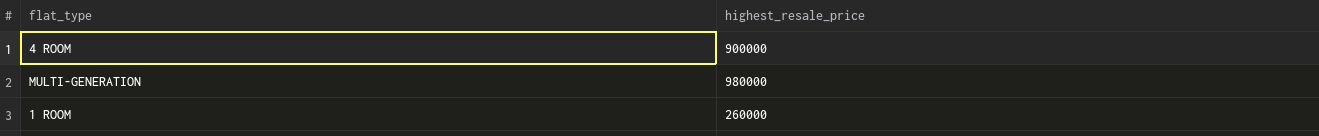
\includegraphics[width=150mm]{hvalpertype-data.png}

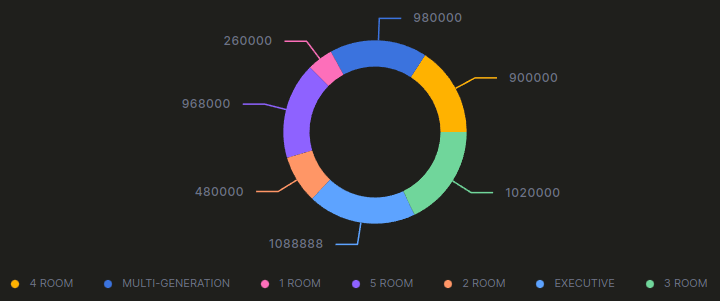
\includegraphics[width=150mm]{hvalpertype.png}
